\documentclass[english, no-theorem-numbers]{short-notes}

\usepackage{math-alg,math-ag}

\addbibresource{math.bib}
%\bibliography{math.bib}

\title{Spectral geometry of Hecke algebras and traces}
\author{David Nadler\\ Lecture notes by Clemens Koppensteiner}
\date{July 1--8, 2013}
\version{0}

\begin{document}

\newcommand\Sing{\operatorname{Sing}}
\newcommand\Loc{\operatorname{Loc}}
\newcommand\K{\sheaf K}%
\newcommand\ld[1]{\check{#1}}
\renewcommand\Gr{\operatorname{Gr}}

\maketitle

\tableofcontents
\bigskip\noindent
By geometry we mean that we work in the function field case, with a base field $k$ of characteristic $0$.

\section{Derived algebraic geometry}

While algebraic geometers ostensibly study solutions to polynomial equations, it has been long known that it is important to keep track of the actual equations instead of merely their solutions.
Hence we can say that Algebraic Geometry is the study of \emph{systems} of polynomial equations.
An example of our slogan \enquote{equations over solutions} is the importance of nilpotents.

General references for this section are the works of Toën--Vezzosi and Lurie.

\subsection{Three examples of \enquote{derived equations}}

\subsubsection{Intersection multiplicities}

Consider $\as 4 = \Spec k[x,y,z,w]$ and the subvarieties $X₁ = \{x = y = 0\} \cup \{z=w=0\} = \{xz=xw=yz=yw\}$ and $X₂ = \{x = z,\, y = w\}$.
Obviously, $X₁ \cap X₂ = \{0\}$.
However, if we perturb $X₂$ by a little bit, we get two points.

If we impose all equations for $X₁\cap X₂$, then we get $x² = xy = xy = y²$.
Note that we get $xy$ in two different ways: from $xw = 0$, $y = w$ and from $yz = 0$, $x = z$.
Thus the dimension of $\O_{X₁ \cap X₂}$ is $3$ instead of the expected $2$ in the perturbed, \enquote{transversal} situation.
Serre's intersection multiplicity formula tells us that 
\[ 2 = 3 - 1, \]
where the $1$ is the dimension of a $\Tor$.

\subsubsection{Base change}

Consider a Cartesian diagram
\[
    \begin{tikzpicture}
        \matrix[commutative diagram] (m) {
            X₁ ×_Y X₂ & X₂ \\
            X₁ & Y \\
        };
        \path[commutative diagram arrows]
            (m-1-1) edge node[above] {$p₂$} (m-1-2)
                    edge node[left] {$p₁$} (m-2-1)
            (m-1-2) edge node[right] {$f₂$} (m-2-2)
            (m-2-1) edge node[below] {$f₂$} (m-2-2);
    \end{tikzpicture}
\]
Base change is the statement that ${p₂}_*p₁^* = f₂^*{f₁}_*$ as functors $\catCoh{X₁} → \catCoh{X₂}$.
Here and in the rest of the document all categories of modules and all functors between them are automatically derived, even when not explicitly mentioned in the notation.

Unfortunately, base change fails even in simple situations.
\begin{Ex}
    Consider the diagram 
    \[
        \begin{tikzpicture}
            \matrix[commutative diagram] (m) {
                \{0\} ×_{\as 1} \{0\} & \{0\} \\
                \{0\} & \as 1 \\
            };
            \path[commutative diagram arrows]
            (m-1-1) edge (m-1-2)
                    edge (m-2-1)
            (m-1-2) edge (m-2-2)
            (m-2-1) edge (m-2-2);
        \end{tikzpicture}
    \]
    Classically, the upper left corner is simply equal to $\{0\}$ again.
    The functor $\catModules{k} → \catModules{k}$ around the upper left part of the diagram is simply the identity, while the functor around the lower right is given by tensoring with the complex $k[1]\oplus k$.
    Derived algebraic geometry will change the upper functor ($\id$ in this case) by changing the fiber product.
\end{Ex}

\begin{Exercise}
    Let $Q^3 = \{A ∈ M₂ : \det A = 0\}$.
    This has two canonical resolutions $Q^3_+$ and $Q³_-$ given by adding a line in the kernel or cokernel of the matrix (they are a basic example of a \enquote{flop}).
    Find the correct (derived) fiber product $\tilde Q = Q³_+ ×_{Q³} Q³_-$, so that base change holds.
    (You will need material discussed later in this section to do the exercise.)
\end{Exercise}

\subsubsection{Moduli problems}

Classically there are strange ambiguities, in particular for deformations.

\begin{Ex}
    Let $\mathcal M_n$ be the moduli space of two commuting operators on $k^n$.
    We can write $\mathcal M_n$ as a fiber product
    \[
        \begin{tikzpicture}
            \matrix[commutative diagram] (m) {
                \mathcal M_n & M_n^2 \\
                \{0\} & M_n \\
            };
            \path[commutative diagram arrows]
            (m-1-1) edge (m-1-2)
                    edge (m-2-1)
            (m-1-2) edge node[right] {$[\,{,}\,]$} (m-2-2)
            (m-2-1) edge (m-2-2);
        \end{tikzpicture}
    \]
    For $n = 1$ we obtain
    \[
        \begin{tikzpicture}
            \matrix[commutative diagram] (m) {
                \mathcal M₁ & \as 1 × \as 1 \\
                \{0\} & M₁ \\
            };
            \path[commutative diagram arrows]
            (m-1-1) edge (m-1-2)
                    edge (m-2-1)
            (m-1-2) edge node[right] {$[\,{,}\,]$} (m-2-2)
            (m-2-1) edge (m-2-2);
        \end{tikzpicture}
    \]
    and, since any two matrices in $M₁$ commute, that $\mathcal M₁ = \as 1 × \as 1$.
    But if we deform slightly and require that $[\,{,}\,] = λ \ne 0$, then the moduli space suddenly becomes empty!
\end{Ex}

\subsection{Local (affine) DAG}

Imposing equations translates to tensor products and in a derived setting this means that we have to keep track of $\Tor$s.

\begin{Def}
    A \emph{commutative differential-graded algebra} (\emph{cdga}) $A^\cx$ over $tk$ is a commutative, associative algebra in $k$-chain complexes.
\end{Def}

\begin{Rem}
    We consider cdgas only up to quasi-isomorphism, but be aware that $A^\cx$ knows more that $H^\cx(A^\cx)$.
\end{Rem}

\begin{Exercise}
    Give an example of two cdgas with the same cohomology algebra (hint: Massey products).
\end{Exercise}

\begin{Def}
    A \emph{derived ring} $A^\cx$ is a cdga which is connective, i.e.~$H^iA^\cx = 0$ for $i > 0$.
    The opposite category to derived rings is called the category of \emph{affine derived schemes}.
\end{Def}

\begin{Notation}
    We often write $π_i = H^{-i}$.
\end{Notation}

\begin{Rem}
    We have a canonical map $A^\cx → π₀A^\cx$.
    Hence we can view $A^\cx$ as a \enquote{derived thickening} of $π₀A^\cx$.
    On schemes, we see this as an embedding $\Spec π₀A^\cx \hookrightarrow \Spec A^\cx$.
\end{Rem}

The source of all examples for derived rings are iterated fiber products where we keep track of $\Tor$ complexes.

\subsubsection{Structure of cdgas}

The category of cdgas should be properly viewed as an $∞$-category and is a simplicial localization of a model category.
The main structure are simplicial sets of $\Hom$:
\[
    \Hom^n(A,B) = \Hom^0(A, B \otimes Ω^\cx(Δ^n)).
\]
Practically, to calculate derived operations we only need to know the following:
\begin{enumerate}
    \item All objects are fibrant.
    \item Cell cdgas are cofibrant.
\end{enumerate}

\begin{Def}
    A cdga $A$ is a \emph{cell cdga} if it has a filtration
    \[
        k = A_0 \hookrightarrow A₁ \hookrightarrow A₂ \hookrightarrow \dotsb \hookrightarrow A_n = A,
    \]
    such that $A_{i+1} = A_i[x_i]$ with $\deg x_i ∈ ℤ$ and $dx_i ∈ A_i$.
    \todo{Is this the same as semifree algebras?}%
    \todo{Rather than $k$ should we start with the algebra over which we are taking the tensor product?}%
\end{Def}

\begin{Ex}
    Consider a hypersurface $X = \{f = 0\}$ in $\as n$.
    Traditionally we have $\O(X) = \rquot{k[x₁,\dotsc,x_n]}{(f)}$.
    The cofibrant replacement of this is $k[x₁,\dotsc,x_n][ε]$ with $\deg ε = -1$ (and hence $ε²=0$) and $dε = f$.
\end{Ex}

\subsubsection{Linearization}

Let $A$ be a derived ring.

\paragraph{Modules}
Attached to $A$ are various categories of modules, which are summarized in Figure~\ref{fig:modules}.
\begin{figure}[htb]
    \centering
    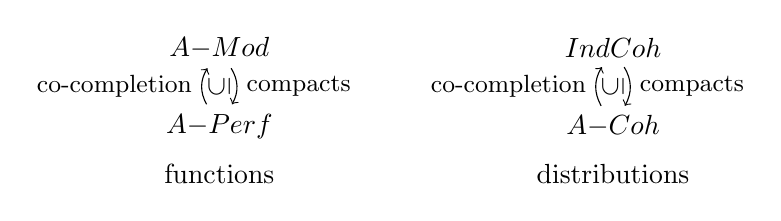
\begin{tikzpicture}
        \node (QCoh) at (0,0) {$A\text{-}\cat{Mod}$};
        \node at (0,-0.5) [rotate=90] {$\subseteq$};
        \node (Perf) at (0,-1) {$A\text{-}\cat{Perf}$};
        \draw[->] (Perf) to[bend left=30] node[left] {\small co-completion} (QCoh);
        \draw[->] (QCoh) to[bend left=30] node[right] {\small compacts} (Perf);
        \node at (0,-1.6) {\enquote{functions}};
        \begin{scope}[xshift={5cm}]
            \node (IndCoh) at (0,0) {$\cat{IndCoh}$};
            \node at (0,-0.5) [rotate=90] {$\subseteq$};
            \node (Coh) at (0,-1) {$A\text{-}\cat{Coh}$};
            \draw[->] (Coh) to[bend left=30] node[left] {\small co-completion} (IndCoh);
            \draw[->] (IndCoh) to[bend left=30] node[right] {\small compacts} (Coh);
            \node at (0,-1.6) {\enquote{distributions}};
        \end{scope}
    \end{tikzpicture}
    \caption{Categories of modules attached to a derived ring.}
    \label{fig:modules}
\end{figure}
\begin{itemize}
    \item $A\text{-}\cat{Mod}$ is the category of derived dg modules.
    \item $A\text{-}\cat{Perf}$ the subcategory consisting of summands of finite complexes of shifts of $A$.
    \item $\cat{IndCoh}$ is the category of ind-coherent modules.
    \item $A\text{-}\cat{Coh}$ is the subcategory of $A\text{-}\cat{Mod}$ consisting of complexes with bounded coherent cohomology.
\end{itemize}

\paragraph{Cotangent complex}
To $A$ we attach its \emph{cotangent complex} $\mathbb L_A ∈ A\text{-}\cat{Mod}$, which is a connective module such that $π₀\mathbb L_A$ coincides with the cotangent bundle $Ω_{π₀A}$.
The universal characterization of the cotangent complex is 
\[
    \operatorname{Der}(A,M) = \Hom(\mathbb L_A, M).    
\]
In particular we have a \enquote{Kähler differential} $d\colon A → \mathbb L_A$.

To calculate we only need to know that $\mathbb L_A$ coincides with the cotangent bundle on smooth classical affine schemes and if $D = A \otimes_C^{\mathbb L} B$, then
\[
    \mathbb L_D = \operatorname{Cone}\left( \mathbb L_A \otimes_A D → (\mathbb L_B \otimes_B D) \oplus (\mathbb L_C \otimes_C D) \right),
\]
where the map is given by pullback.

\subsection{Global DAG}

We take the functor of points viewpoint:
\[
    \begin{tikzpicture}
        \matrix[commutative diagram] (m) {
            \cat{Aff}^{\mathrm{op}} & \cat{Sets} \\
            \cat{DAff}^{\mathrm{op}} & \cat{Spaces} = \cat{SSet} \\
        };

        \path[->] 
            (m-1-1) edge node[above] {Sch} (m-1-2)
                    edge node[auto,sloped,anchor={south}] {Stacks} (m-2-2)
            (m-2-1) edge node[below] {DStacks} (m-2-2);
        \path[right hook->]
            (m-1-1) edge (m-2-1)
            (m-1-2) edge (m-2-2);
    \end{tikzpicture}
\]
In particular, Artin derived stack are given by a diagram of the form
\[
    X \leftarrow \left(X₀ \leftleftarrows X₁\right),
\]
where $X₀$ and $X₁$ are derived schemes and the two arrows $\leftleftarrows$ are smooth maps.

\begin{Ex}\leavevmode
    \begin{enumerate}
        \item $BG \leftarrow (\mathrm{pt} \leftleftarrows G$), for $G$ a group.
        \item $M_{1,1} \leftarrow (? \leftleftarrows ?)$.
        \item $S¹ \leftarrow (\mathrm{pt} \leftleftarrows ℤ)$.
            \qedhere
    \end{enumerate}
\end{Ex}

\section{Microlocal algebraic geometry}

The goal of this section is to introduce geometric Arthur parameters. 
There is work by many people on the ideas we will introduce, but the \enquote{state of the art} is \cite{ArinkinGaitsgory:arXiv:SingularSupport}.

We will work locally and set $X = \{F = 0\}$, where $F\colon \as n → \as k$.
We want to understand the (derived) category $\catCoh X$.

\subsection{Philosophy: two themes}

The ideas we will introduced a based on two major themes in mathematics. 
The first of these is illustrated by the following example.

\begin{Ex}
    Let $A$ be an algebra and consider the category $\catModules A$ of $A$-modules.
    Let $Z(A)$ be the center of $A$.
    Then $\Spec Z(A)$ is a scheme, and we can localize $A$ as a sheaf of algebras on $\Spec Z(A)$.
    Therefore we can localize the category $\catModules A$ on $\Spec Z(A)$.
\end{Ex}

More generally, if $\cat C$ is a category, we can sheafify $\cat C$ over $Z(\cat C) = \End(\id[\cat{C}])$.

The second theme is that there are two types of \enquote{geometric measurements}: 
\begin{itemize}
    \item static measurements corresponding to points of $X$, e.g.~talking stalks;
    \item dynamic measurements corresponding to $T^*X$, e.g.~taking vanishing cycles.
\end{itemize}

A classical example is Fourier transform $L²(S¹) \isoto L²(ℤ)$.

\subsection{Koszul duality}

Let $V = \Spec k[x₁,\dotsc,x_n]$ with $\deg x_i = -1$ be a \enquote{vector space in degree $-1$.}
We want to analyze $\catCoh V$.

Note that $V_{\mathrm{cl}} = \Spec π₀V$ is just a point, so that this doesn't give us any way to localize.
Thus we introduce \emph{codirections} $V^*[1] = \Spec k[ξ₁,\dotsc,ξ_n]$ with $\deg ξ_i = 2$.

\begin{Thm}[Koszul Duality]
    There is an equivalence of categories
    \[
        \catCoh V \cong \catCoh{V^*[1]},
    \]
    sending the structure sheaf $\O_V$ to the skyscraper $k$ on $V^*[1]$ and the skyscraper $k$ on $V$ to $\O_{V^*[1]}$.
\end{Thm}

Thus we can localize coherent sheaves on $V$ on $V^*[1]$ (which is given by a \enquote{usual} polynomial ring).
Supports will be closed conic subvarieties.

\begin{Exercise}
    Under Koszul Duality, $\sheaf F ∈ \catCoh V$ is perfect if and only if $\supp F \subseteq \{0\} \subseteq V^*[1]$.
\end{Exercise}

\begin{Rem}
    We think of $\catCoh V$ as \enquote{distributions} and $\catPerf V \subseteq \catCoh V$ as \enquote{functions}.
    Koszul Duality measures the codirections on which \enquote{smoothness} fails.
\end{Rem}

\begin{Exercise}
    Show that $V = \{0\} ×_{\as n} \{0\}$ as derived schemes.
    Thus $V$ is an Abelian groupoid via \enquote{concatenation of paths}.
    This turns $\catCoh V$ into a tensor category with tensor product $*$ given by convolution.
    Show that Koszul Duality is an equivalence of tensor categories exchanging $*$ with the usual tensor product $\otimes$ in $\catCoh{V^*[1]}$.
\end{Exercise}

\subsection{The scheme of singularities}

Let us return to the situation of $X = \{F = 0\} \subseteq \as n$.
The cotangent complex of $X$ is given by
\[
    \mathbb L_X = \left( Ω_{\as k} \xrightarrow{dF^*} Ω_{\as n} \right)
\]
in degrees $-1$ and $0$.

\begin{Def}
    The (classical) scheme $\Sing(X) → X$ is the scheme with fiber at $x ∈ X$ given by $H^{-1}\mathbb L_X$.
\end{Def}

\begin{Ex}
    Consider $X = \{x³ = y²\}$.
    Then $\Sing(X)$ is the whole picture given in Figure~\ref{fig:SingEx}.
    \begin{figure}[htb]
        \centering
        \begin{tikzpicture}
            \draw plot[smooth] file {cusp.table};
            \draw[y=-1cm] plot[smooth] file {cusp.table};
            \draw (-1,0) -- (1.5,0);
        \end{tikzpicture}
        \caption{Scheme of singularities of $x³ = y²$}
        \label{fig:SingEx}
    \end{figure}
\end{Ex}

\begin{Rem}
    We always have $\Sing X \subseteq X × \as k$.
\end{Rem}

We can then localize $\catCoh X$ over $\Sing(X)$.

\begin{Rem}
    This will be the ultimate localization.
\end{Rem}

To do so, we need do find the action of $\O(\as k) = k[ξ₁,\dotsc,ξ_k]$.
Consider the Cartesian diagrams (in derived schemes)
\[
    \begin{tikzpicture}
        \matrix[commutative diagram] (m) {
            X & \as n \\
            \{0\} & \as k \\
        };
        \path[commutative diagram arrows]
            (m-1-1) edge (m-1-2) edge (m-2-1)
            (m-1-2) edge node[right] {$F$} (m-2-2)
            (m-2-1) edge (m-2-2);

        \begin{scope}[xshift={4cm}]
            \matrix[commutative diagram] (m) {
                V & \{0\} \\
                \{0\} & \as k \\
            };
            \path[commutative diagram arrows]
                (m-1-1) edge (m-1-2) edge (m-2-1)
                (m-1-2) edge (m-2-2)
                (m-2-1) edge (m-2-2);
        \end{scope}
    \end{tikzpicture}
\]
We should think of points of $X$ as paths from $F$ to $\{0\}$ and points in $V$ as loops based at $\{0\}$.
Thus we can concatenate such a path with a loop and get another path.

The upshot of this is that we have an action of $\catCoh V$ on $\catCoh X$.
The unit of the convolution product $*$ of $\catCoh V$ is $k$.
Hence we obtain a map
\[
    k[ξ₁,\dotsc,ξ_k] = \End(k) → \End(\id[\catCoh X]).
\]
In other words, $k[ξ₁,\dotsc,ξ_k]$ acts universally on every object of $\catCoh X$.
Hence $\catCoh X$ can be localized on $X × \as n$.

\begin{Exercise}
    The support of any element of $\catCoh X$ will always be contained in $\Sing(X)$.
\end{Exercise}

\begin{Ex}
    Let $Q³ = \{A ∈ M₂ : \det A = 0\}$.
    This can be presented as
    \[
    \begin{tikzpicture}
        \matrix[commutative diagram] (m) {
            Q³ & \as 4 \\
            \{0\} & \as 1 \\
        };
        \path[commutative diagram arrows]
            (m-1-1) edge (m-1-2) edge (m-2-1)
            (m-1-2) edge node[right] {$\det$} (m-2-2)
            (m-2-1) edge (m-2-2);
    \end{tikzpicture}
    \]
    and $\Sing(X) \subseteq X × \as 1$ is $X$ together with a one-dimensional \enquote{spoke} at the origin.
\end{Ex}

\begin{Exercise}
    Let $\sheaf F ∈ \catCoh X$.
    Show that $\supp \sheaf F \subseteq \{0\} \subseteq \Sing(X)$ if and only if $\sheaf F ∈ \catPerf X$.
\end{Exercise}

\subsection{Geometric Arthur parameters}

Let $C$ be a smooth projective curve over $k$.
We are interested in $\Loc_G(C)$, the moduli of local $G$-systems on $C$.
There are two versions of what this could mean, but for now we will only consider the \enquote{Betti version}
\[
    \Loc_G(C) = \rquot{\left\{ π₁C → G  \right\}}{C}.
\]
The stack $\Loc_G(C)$ has a presentation
\[
    \Loc_G(C) \leftarrow \left( \Loc_G(C)' \leftleftarrows G \right),
\]
where $\Loc_G(C)'$ is given by \todo{What is the meaning of $\Loc_G(C)'$?}
\[
    \begin{tikzpicture}
        \matrix[commutative diagram] (m) {
            \Loc_G(C)' & G^{2g} \\
            \{1\} & G \\
        };
        \path[commutative diagram arrows]
            (m-1-1) edge (m-1-2) edge (m-2-1)
            (m-1-2) edge node[right] {$[\,{,}\,]$} (m-2-2)
            (m-2-1) edge (m-2-2);
    \end{tikzpicture}
\]
We call $\Sing(\Loc_G(C)) \subseteq \rquot{(\Loc_G(C)' × \liealg g^*)}{G}$ the \emph{moduli of geometric Arthur's parameters}.
One expects that automorphic objects lead to coherent sheaves with nilpotent Arthur's parameters.

\section{Hecke categories}

Let $G$ be a reductive group and recall that the spherical Hecke algebra of $G$ is defined as
\[
    H_{\mathrm{sph}} = ℂ_c\left[ \dquot{G(ℤ_p)}{G(ℚ_p)}{G(ℤ_p)} \right].
\]
Attached to $G$ is its root datum
\[
    \left( Λ_G,\, \ld{Λ}_G,\, R_G, \ld R_G \right),
\]
consisting of the coweight lattice, the weight lattice, the coroots and the roots of $G$.
Switching weights and coweights and roots and coroots, we obtain the Langlands dual group $\ld G$ of $G$.
Recall that the Satake isomorphism is an isomorphism 
\[
    H_{\mathrm{sph}} \cong \O(\ld G)^{\ld G}
\]
of commutative algebras between the Hecke category of $G$ (with $*$) and the representation ring of $\ld G$ (with $\cdot$).
The goal of this lecture is to discuss a geometric version of the Satake isomorphism.

\subsection{The affine Grassmannian}

Let $k = ℂ$ (though the construction also works for other fields).

We set $\K = k\lParen t \rParen$ be the ring of Laurent series over $k$ and $\O = k\lBrack t \rBrack$ its subring of power series.
We think of $\Spec \O$ as a formal disc and $\Spec \K$ as a punctured formal disc.
Thus we call $LG = G(\K)$ the \emph{loop group} and $L_+G = G(\O)$ the \emph{arc group}.
For example, if $G = \GL n$, then $G(\K)$ consists of invertible matrices with coefficients in $\K$.

\begin{Def}
    The \emph{affine Grassmannian} (or \emph{loop Grassmannian}) is
    \[
        \Gr = \Gr_G = \rquot{LG}{L_+G}.
    \]
\end{Def}

The affine Grassmannian is an increasing union of projective varieties.

\begin{Ex}
    Let $G = \GL n$.
    Then we have an action of $L\GL n$ on $\K^n$.
    The basic lattice $\O^n \subseteq \K^n$ (see Figure~\ref{fig:GLnlattice}) is preserved by $L_+\GL n$.
    \begin{figure}[htb]
        \centering
        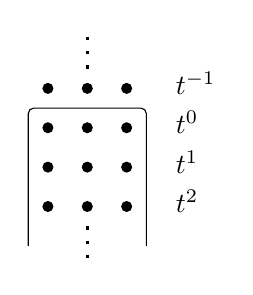
\begin{tikzpicture}[y={-0.5cm}, x={0.5cm}]
            \foreach \i in {-1,0,1,2} {
                \foreach \j in {-1,0,1} {
                    \fill ({\j},{\i}) circle[radius=2pt];
                }
                \node[anchor=mid west] at (2,\i) {$t^{\i}$};
            }
            \draw[rounded corners=2pt] (-1.5,3) -- (-1.5,-0.5) -- (1.5,-0.5) -- (1.5,3);
            \draw[loosely dotted, very thick] (0,-1.5) -- (0,-2.5);
            \draw[loosely dotted, very thick] (0,2.5) -- (0,3.5);
        \end{tikzpicture}
        \caption{The lattice of basis vectors of $\K^3$ after fixing a basis for $ℂ³$ with the basic lattice $\O^n$ marked.}
        \label{fig:GLnlattice}
    \end{figure}
    \begin{Exercise}
        Show that 
        \[
            \Gr_{\GL n} = 
            \left\{ 
                \text{$k$-subspaces $W \subseteq \K^n$ such that $tW \subseteq W$ and $t^N\O^n \subseteq W \subseteq t^{-N}\O^n$ for $N \gg 0$}
            \right\}.
        \]
    \end{Exercise}
    Hence we can write $\Gr_{\GL n} = \smash{\bigcup\limits_{\mathclap{N = 0}}^∞ \Gr_N}$, where
    \[
        \Gr_N = 
        \left\{ 
            \text{$k$-subspaces $W \subseteq \K^n$ such that $tW \subseteq W$ and $t^N\O^n \subseteq W \subseteq t^{-N}\O^n$}
        \right\}.
    \]
    is a projective variety.
    \begin{figure}[htb]
        \centering
        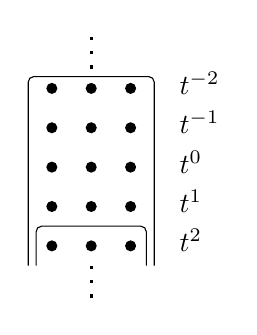
\begin{tikzpicture}[y={-0.5cm}, x={0.5cm}]
            \foreach \i in {-2,-1,0,1,2} {
                \foreach \j in {-1,0,1} {
                    \fill ({\j},{\i}) circle[radius=2pt];
                }
                \node[anchor=mid west] at (2,\i) {$t^{\i}$};
            }
            \draw[rounded corners=2pt] (-1.6,2.5) -- (-1.6,-2.3) -- (1.6,-2.3) -- (1.6,2.5);
            \draw[rounded corners=2pt] (-1.4,2.5) -- (-1.4,1.5) -- (1.4,1.5) -- (1.4,2.5);
            \draw[loosely dotted, very thick] (0,-2.5) -- (0,-3.5);
            \draw[loosely dotted, very thick] (0,2.5) -- (0,3.5);
        \end{tikzpicture}
        \caption{The bounds for $W$ in $\Gr_2$.}
        \label{fig:GLnlatticeN}
    \end{figure}
\end{Ex}

\subsection{Alternative descriptions}

\subsubsection{Bundles}

Let $D = \Spec \O$ and $D^× = \Spec \K$.
Then $\Gr$ is the set of $G$-bundles on $D$, trivialized on $D^×$.
Hence, if $\mathbb D = D \amalg_{D^×} D$ is the disc with two origins, we have
\[
    \lquot{L_+G}{\Gr} =
    \dquot{L_+G}{LG}{L_+G} = 
    \{ \text{$G$-bundles on $\mathbb D$}\}.
\]

\subsubsection{Topological}

Let $K \subseteq G$ be a maximal compact and let $ΩK$ be the based polynomial\footnote{I.e., as maps $S¹ → K$ the loops have finite Fourier expansion} loop group on $K$.
Then
\[ \Gr \cong ΩK\]
as topological spaces.
In fact, $LG \cong ΩK × L_+G$.

\begin{Exercise}
    Show that for $G = \PGL 2$ one has
    \[
        \Gr_{\PGL 2} = \rquot{\operatorname{Free}(S²)}{xa(x) = 1},
    \]
    where $\operatorname{Free}(X)$ denotes the free topological group on $X$ and $a\colon S² → S²$ is the antipodal map.
\end{Exercise}

\section{Geometric traces}

\printbibliography
\end{document}
